\documentclass{article}

\usepackage{graphicx}
\usepackage{tikz}
\usepackage{tikzsymbols}
\usetikzlibrary{calc,patterns,shapes.geometric}
\pagestyle{empty}
\usepackage[margin=0pt]{geometry}
\geometry{papersize={14in,12in}}

\def\centerarc[#1](#2)(#3:#4:#5){\draw[#1] ($(#2)+({#5*cos(#3)},{#5*sin(#3)})$) arc (#3:#4:#5);}

\begin{document}
	\begin{figure}
		\centering
		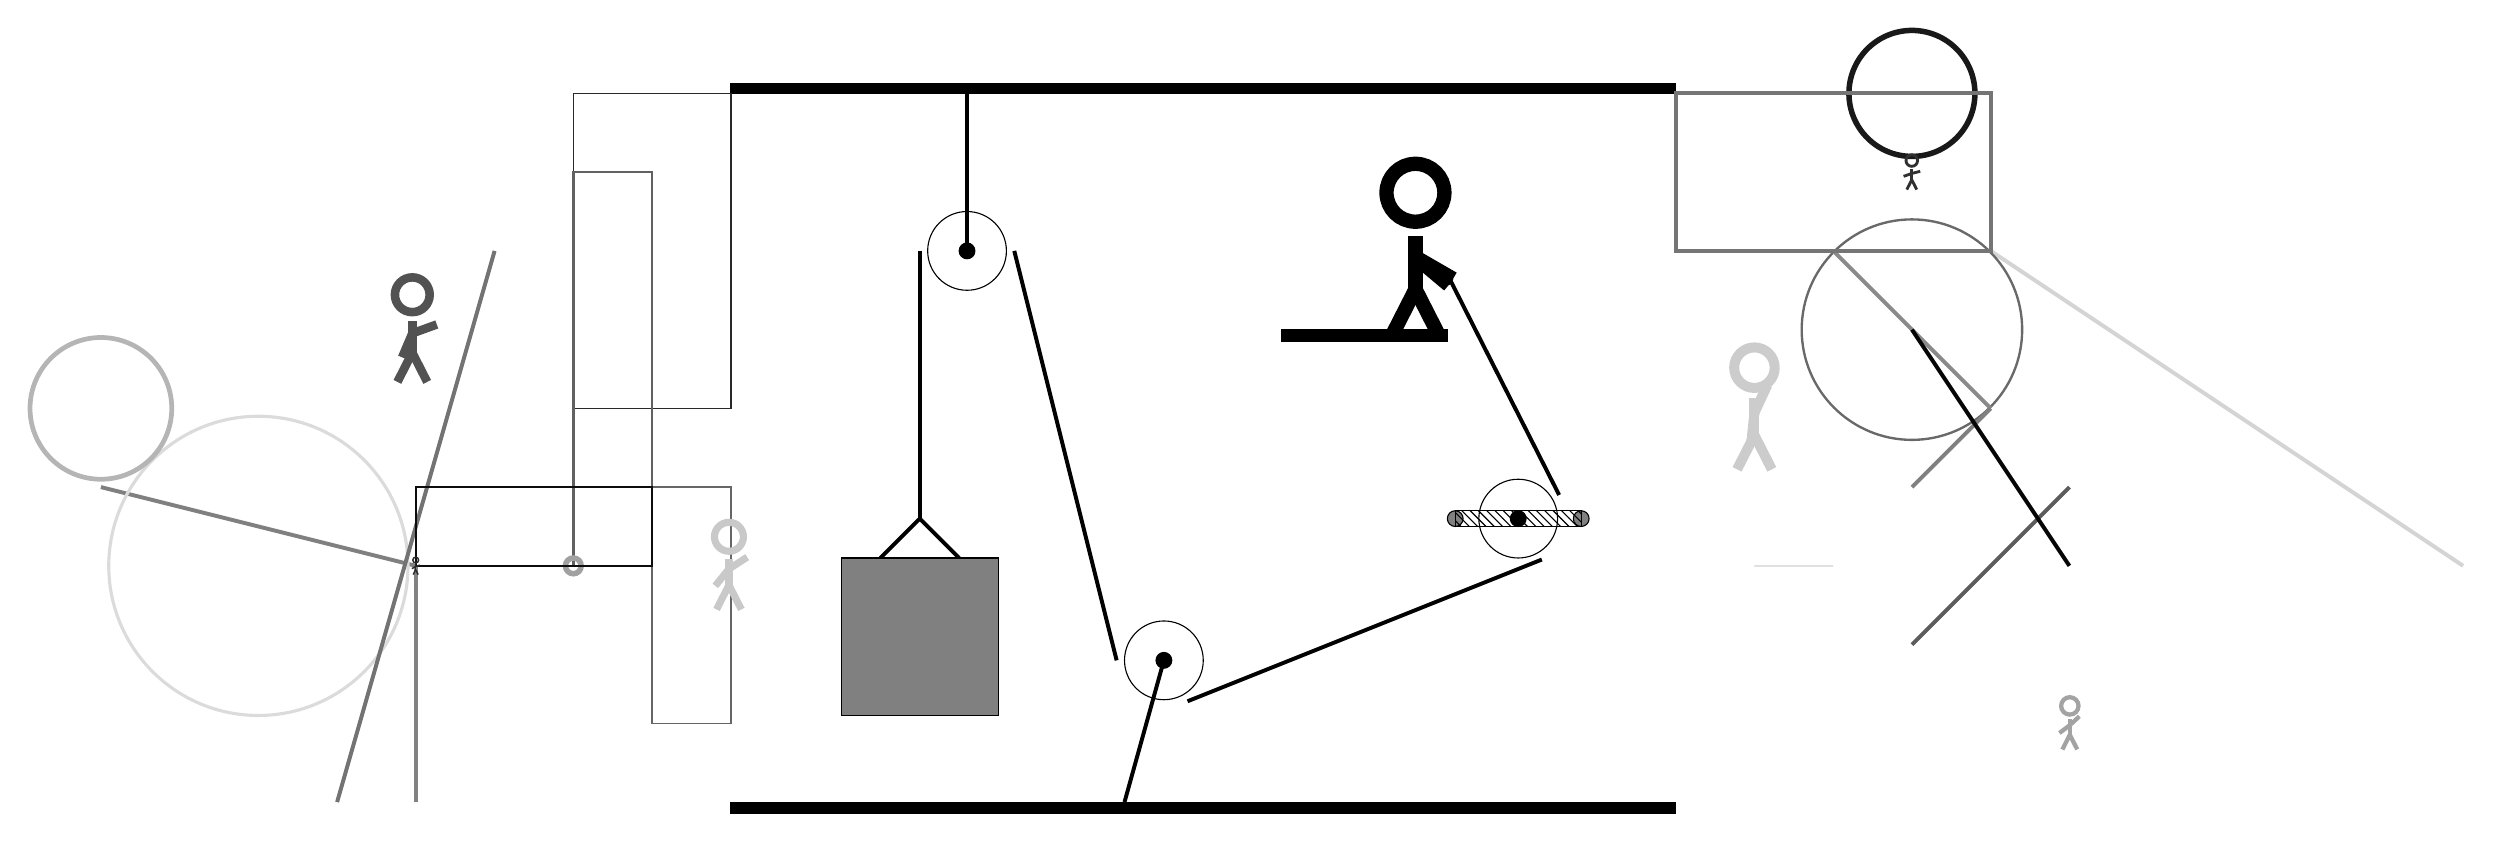
\begin{tikzpicture}
			%%%%% START %%%%%
			
			\draw[fill=black] (-2, 9) rectangle (10, 9.125);
			
			\draw (1, 7) circle (0.5);
			\draw[fill=black] (1, 7) circle (0.1);
			\draw[line width=0.5mm] (1, 9) -- (1, 7);
			
			\draw (3.5, 1.8) circle (0.5);
			\draw[fill=black] (3.5, 1.8) circle (0.1);
			\draw[line width=0.5mm] (3.5, 1.8) -- (3.0, 0);
			
			\draw[fill=white](8, 3.6) circle (0.5);
			\draw[fill=black] (8, 3.6) circle (0.1);
			\draw[fill=black!50] (8.8, 3.6) circle (0.1);
			\draw[fill=black!50] (7.2, 3.6) circle (0.1);
			\draw[pattern=north west lines, pattern color=black] (7.2, 3.7) rectangle (8.8, 3.5);
			
			\draw[line width=0.5mm](-0.1, 3.1) --  (0.4, 3.6) -- (0.9, 3.1);
			\draw[fill=black!50] (-0.6, 3.1) rectangle (1.4, 1.1);
			
			\draw[line width=0.5mm](0.4, 7) -- (0.4, 3.6);
			\centerarc[line width=0.5mm](1, 7)(180:0:0.6)
			\draw[line width=0.5mm](1.6, 7) -- (2.9, 1.8);
			\centerarc[line width=0.5mm](3.5, 1.8)(180:300:0.6);
			\draw[line width=0.5mm](3.8, 1.2804) -- (8.3, 3.0804);
			\centerarc[line width=0.5mm](8, 3.6)(300:390:0.6);
			\draw[line width=0.5mm](8.5196, 3.9) -- (7.05, 6.8);
			
			\node at (6.75, 7) {\Strichmaxerl[10][-220][-30]};
			\draw[fill=black] (5, 6) rectangle (7.1, 5.85);
			
			\draw[line width=0.5mm, color=black!17](14, 7) -- (20, 3);
			
			\draw [line width=0.3mm, color=black!59](13, 6) circle (1.4);
			\draw[line width=0.5mm, color=black!46](14, 5) -- (12, 7);
			\draw[line width=0.5mm, color=black!50](-6, 3) -- (-10, 4);
			
			\draw [line width=0.7mm, color=black!90](13, 9) circle (0.8);
			\draw[line width=0.2mm, color=black!60] (-2, 1) rectangle (-3, 4);
			\node[line width=0.6mm, color=black!81] at (13, 8) {\Strichmaxerl[2][20][14]};
			\draw [line width=0.4mm, color=black!14](-8, 3) circle (1.9);
			\draw[line width=0.5mm, color=black!55](-5, 7) -- (-7, 0);
			\draw[line width=0.5mm, color=black!49](-6, 0) -- (-6, 3);
			\draw[line width=0.2mm, color=black!84] (-2, 9) rectangle (-4, 5);
			\draw[line width=0.3mm, color=black!62] (-4, 8) rectangle (-3, 3);
			\draw [line width=0.7mm, color=black!37](-4, 3) circle (0.1);
			
			\draw[line width=0.5mm, color=black!50](14, 5) -- (13, 4);
			\draw[line width=0.5mm, color=black!64](13, 2) -- (15, 4);
			\node[line width=0.5mm, color=black!21] at (-2, 3) {\Strichmaxerl[5][51][33]};
			\node[line width=0.4mm, color=black!36] at (15, 1) {\Strichmaxerl[3][37][43]};
			\draw[line width=0.2mm, color=black!95] (-3, 3) rectangle (-6, 4);
			\node[line width=0.7mm, color=black!20] at (11, 5) {\Strichmaxerl[7][84][65]};
			\node[line width=0.3mm, color=black!84] at (-6, 3) {\Strichmaxerl[1][30][19]};
			\draw [line width=0.6mm, color=black!29](-10, 5) circle (0.9);
			\draw[line width=0.2mm, color=black!12] (12, 3) rectangle (11, 3);
			\node[line width=0.5mm, color=black!68] at (-6, 6) {\Strichmaxerl[6][67][20]};
			\draw [line width=0.6mm, color=black!63](17, 1) circle (0.0);
			\draw[line width=0.5mm, color=black!98](15, 3) -- (13, 6);
			
			\draw[line width=0.5mm, color=black!54] (10, 9) rectangle (14, 7);
			
			
			\draw[fill=black] (-2, 0) rectangle (10, -0.15);
			
			%%%%% END %%%%%
		\end{tikzpicture}
	\end{figure}	
\end{document}